\chapter{Estudo de caso}
\label{cap:estudodecaso}

Neste trabalho será feito um estudo sobre uma empresa que fornece serviços de hospedagens e também está associada a um 
provedor de internet\footnotemark[1]. 
A empresa possui grande parte de seus clientes localizados na serra do Rio Grande do Sul, sendo que o número de clientes é aproximadamente 9000. 
A sede da empresa está localizada na cidade de Garibaldi, além disso possui quatro filiais no estado, atendendo aproximadamente xx cidades.
Essa empresa, que será o foco deste trabalho, possui aproximadamente xx funcionários.

\footnotetext[1]{É importante salientar que esse provedor utiliza a maior parte dos serviços da empresa, pois possui maior número de clientes.}

Essa empresa oferece serviços pela internet aos seus clientes, que são: hospedagens de sites, banco de dados, \textit{e-mail}, sistemas de gestão, 
\textit{e-mail marketing}, \textit{backup}, \textit{máquinas virtuais}, autenticação \textit{ADSL}, rádio \textit{online} e telefonia.
O provedor associado fornece aos seus clientes acesso à internet via rádio e acesso à internet por meio de fibra óptica.

Sabendo que a empresa atualmente possui redundância de refrigeração e energia. A redundância de refrigeração é composta por três ares-condicionados. 
A redundância de energia é feita através de três \textit{nobreaks}, sendo que dois deles fazem o balanceamento de carga dos servidores e outros 
equipamentos como por exemplo roteadores. Além disso, possui dois geradores para suprir a necessidade de consumo de energia elétrica. 
Assim, essas redundâncias tem como objetivo prover um ambiente físico estável e confiável.

Para ser possível propor uma solução de alta diponibilidade nos servidores é necessário conhecer o cenário atual da empresa, além de selecionar 
os serviços mais críticos para a empresa. Nas próximas seções serão detalhados: o ambiente físico dos servidores, com suas estruturas e suas 
configurações (Seção \ref{section:ambiente}); a estrutura de virtualização, com a relação de servidores físicos e virtuais, e todos os 
serviços fornecidos pela empresa (Seção \ref{section:servicos}); e por fim a seleção dos serviços críticos (Seção \ref{section:servcrit}).

\section{Ambiente físico da empresa}
\label{section:ambiente}

A estrutura atual da empresa é composta por quatorze servidores físicos montados em um \textit{rack} (Figura \ref{fig:servrack}). 
A configuração de \textit{hardware} desses servidores esta listado na Tabela \ref{tab:servfisicos}, que possui o nome do servidor, 
quantidade e modelo de processadores, quantidade e tipo de memória, número de discos e a capacidade unitária, e o modelo do servidor.

\begin{figure}[servrack]
 \centering
 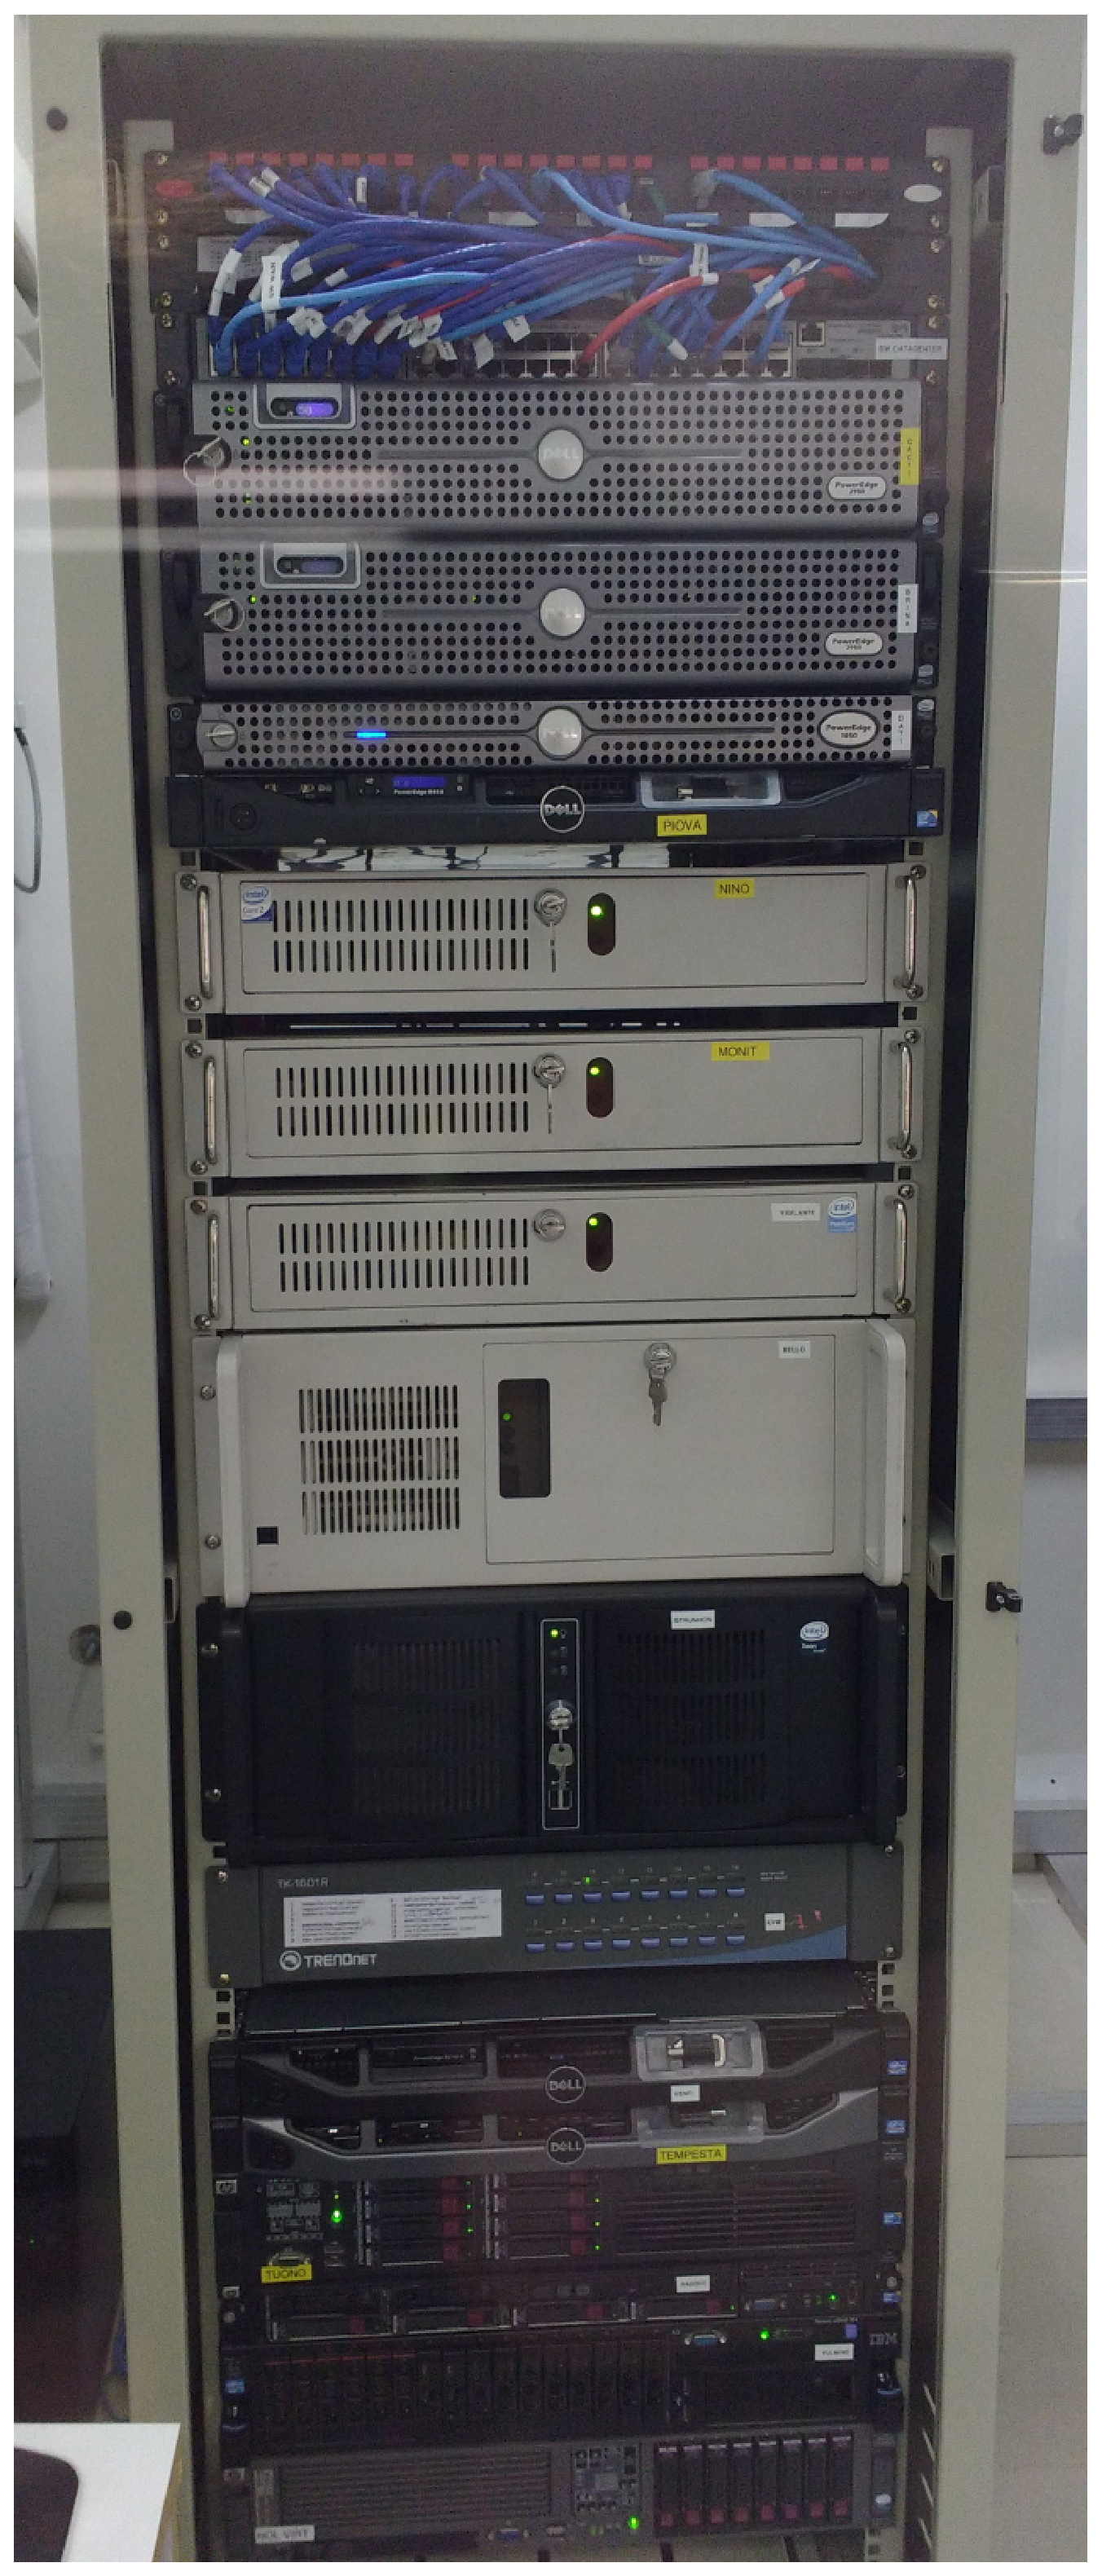
\includegraphics[width=200px]{img/servrack.eps}
 \caption{Imagem do \textit{rack} e dos servidores.}
 \label{fig:servrack}
\end{figure}

\begin{table}
\caption{Configuração dos servidores físicos.}
\label{tab:servfisicos}
\begin{center}
\begin{tabular}{|l|p{4cm}|l|p{2.2cm}|l|}\hline
Servidor & Processador & Memória & Disco & Modelo\\\hline
bello & 1 x Intel Core 2 Duo CPU E6750 2.66 GHz & 2 GB DDR2 & 5,5 TB SATA & \\\hline
brina & 2 x Intel Xeon CPU E5410 2.33 GHz & 24 GB DDR2 & 6 x 300 GB SAS & Dell PowerEdge 2950\\\hline
cacti & 2 x Intel Xeon CPU E5310 1.60 GHz & 12 GB DDR2 & 2 x 73 GB SAS & Dell PowerEdge 2950\\\hline
dati & 2 x Intel Xeon CPU 3.20 GHz & 4 GB DDR2 & 2 x 146 GB SCSI & Dell PowerEdge 1850\\\hline
fulmine & 1 x Intel Xeon CPU E5-2650 2.00 GHz & 32 GB DDR3 & 6 x 2 TB SATA & IBM System x3650 M4\\\hline
monit & 1 x Intel Core 2 Quad CPU Q9550 2.83 GHz & 4 GB DDR2 & 120 GB SSD & \\\hline
nino & 1 x Intel Core 2 Duo CPU E4500 2.20 GHz & 4 GB DDR2 & 500 GB SATA & \\\hline
piova & 2 x Intel Xeon CPU E5530 2.40 GHz & 32 GB DDR3 & 4 x 500G SATA & Dell PowerEdge R410\\\hline
raggio & 2 x  Intel Xeon CPU E5630 2.53 GHz & 32 GB DDR3 & 4 x 300 GB SAS & HP ProLiant DL360 G7\\\hline
sfrunhon & 1 x Intel Xeon CPU X3330 2.66 GHz & 8 GB DDR2 & 750 GB SATA & \\\hline
tempesta & 2 x Intel Xeon CPU E5-2620 2.00 GHz & 32 GB DDR3 & 5 x 1 TB SATA & Dell PowerEdge R620\\\hline
tuono & 2 x Intel Xeon CPU E5649 2.53 GHz & 32 GB DDR3 & 6 x 300 GB SAS 2 x 146 GB SAS & HP ProLiant DL380 G7\\\hline
venti & 1 x Intel Xeon CPU E3-1220 3.10 GHz & 16 GB DDR3 & 2 x 3 TB SATA & Dell PowerEdge R210 II\\\hline
vigilante & 1 x Intel Pentium Dual CPU E2180 2.00 GHz & 4 GB DDR2 & 2,5 TB SATA & \\\hline
\end{tabular}
\end{center}
\end{table}

Os servidores utilizados para virtualização possuem redundância de \textit{hardware}, com fonte de alimentação e discos configurados através 
de um \ac{RAID}.
Além disso, para cada servidor de virtualização dois cabos de rede são ligados a um \textit{switch} \textit{gigabit}, para possibilitar a 
configuração de \textit{link aggregation}, assim caracterizando a redundância do cabeamento e dobrando a capacidade de tráfego de dados.
O diagrama da Figura \ref{fig:servfisicos} demonstra uma visão geral da estrutura física dos servidores da empresa. Todos os servidores 
estão ligados ao \textit{switch}, que provê aos servidores acesso à internet através do roteador. Os servidores de virtualização possuem suas 
respectivas \ac{VM}s, que executam aplicações, e existem servidores que executam aplicações diretamente.

\begin{figure}[servfisicos]
 \centering
 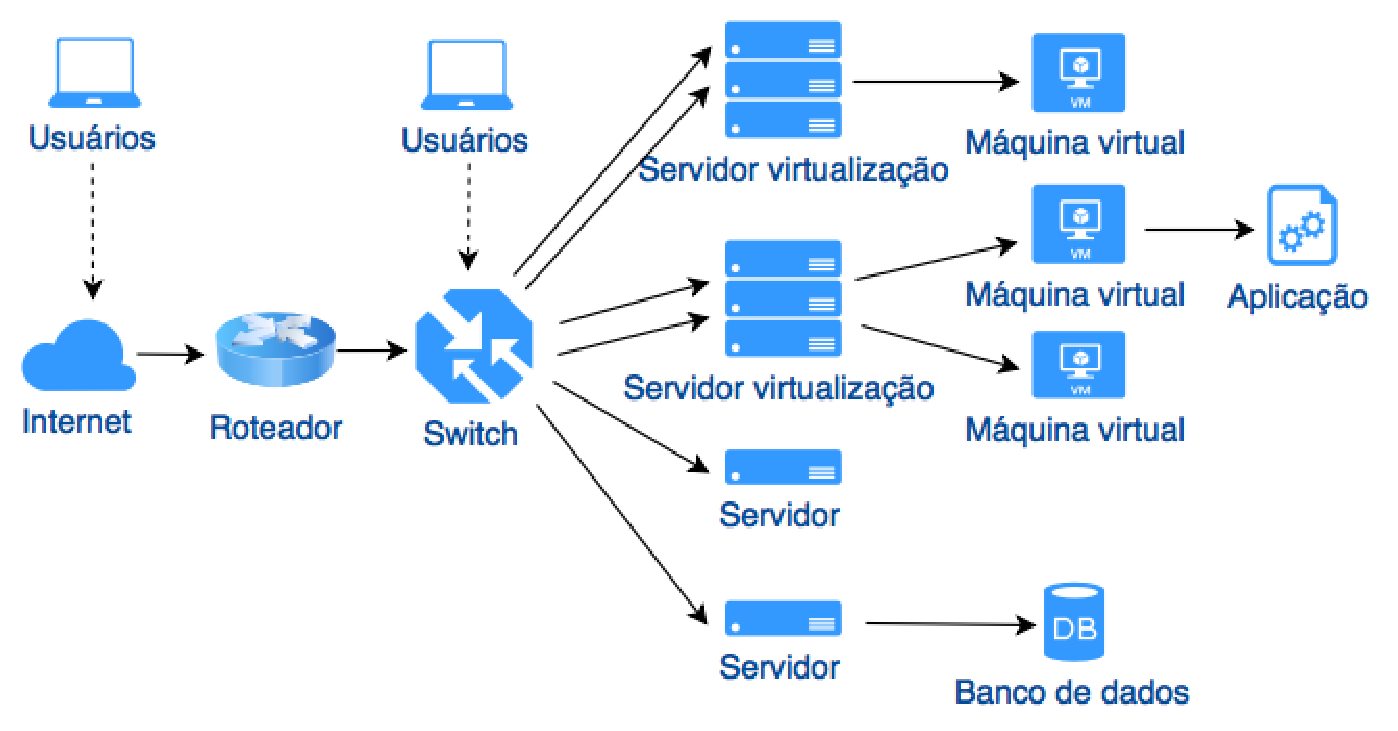
\includegraphics[width=350px]{img/servfisicos.eps}
 \caption{Estrutura física.}
 \label{fig:servfisicos}
\end{figure}

\section{Serviços e virtualização ?}
\label{section:servicos}

A empresa fornece serviços diversos, desde hospedagens de sites até \textit{DNS} recursivo para um provedor de internet. 
Atualmente sete servidores são utilizados com a virtualização, e os outros sete possuem aplicações executando diretamente. 
Sendo que existem quarenta e seis \ac{VM}s distribuídas entre os sete servidores de virtualização, esses servidores são:
\begin{itemize}
 \item Servidor Brina: possui quatro \ac{VM}s, que executam os serviços de ... (Figura \ref{fig:servlog1});
 \item Servidor Fulmine: este executa doze \ac{VM}s (Figura \ref{fig:servlog2}), que executam:
 \begin{itemize}
  \item 
 \end{itemize}
 \item Servidor Piova: 
 \item Servidor Raggio: 
 \item Servidor Tempesta: 
 \item Servidor Tuono: 
 \item Servidor Venti: 
\end{itemize}

\begin{figure}[servlog1]
 \centering
 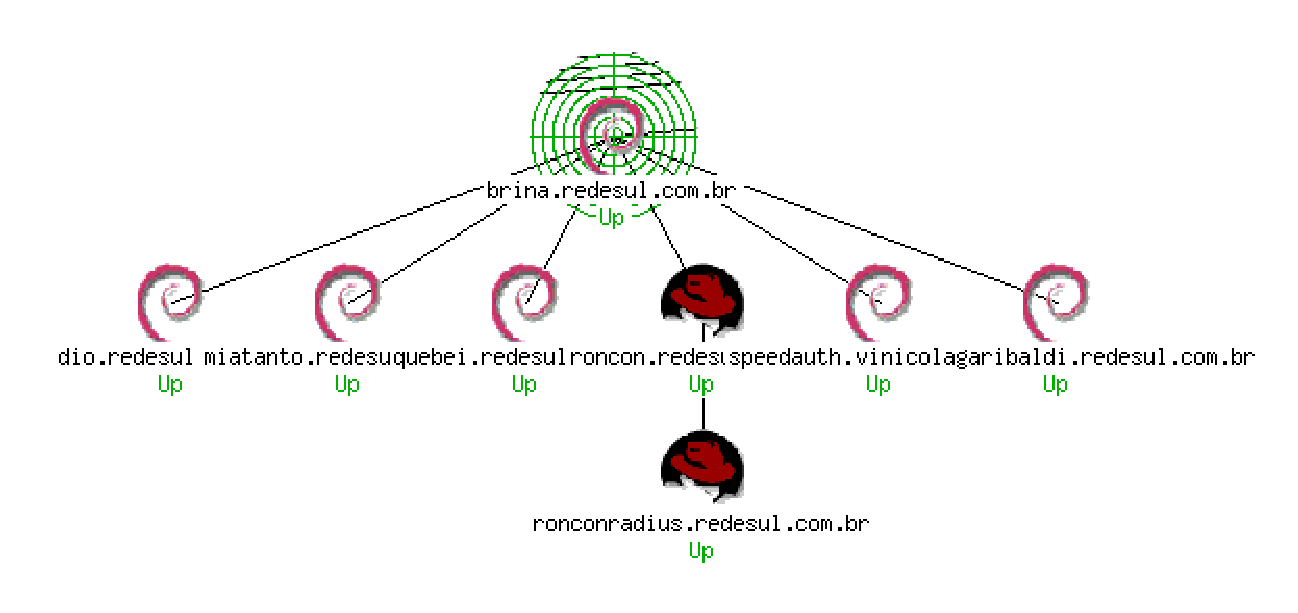
\includegraphics[width=380px]{img/servlog1.eps}
 \caption{Servidor virtualização Brina. REFAZER ???}
 \label{fig:servlog1}
\end{figure}

\begin{figure}[servlog2]
 \centering
 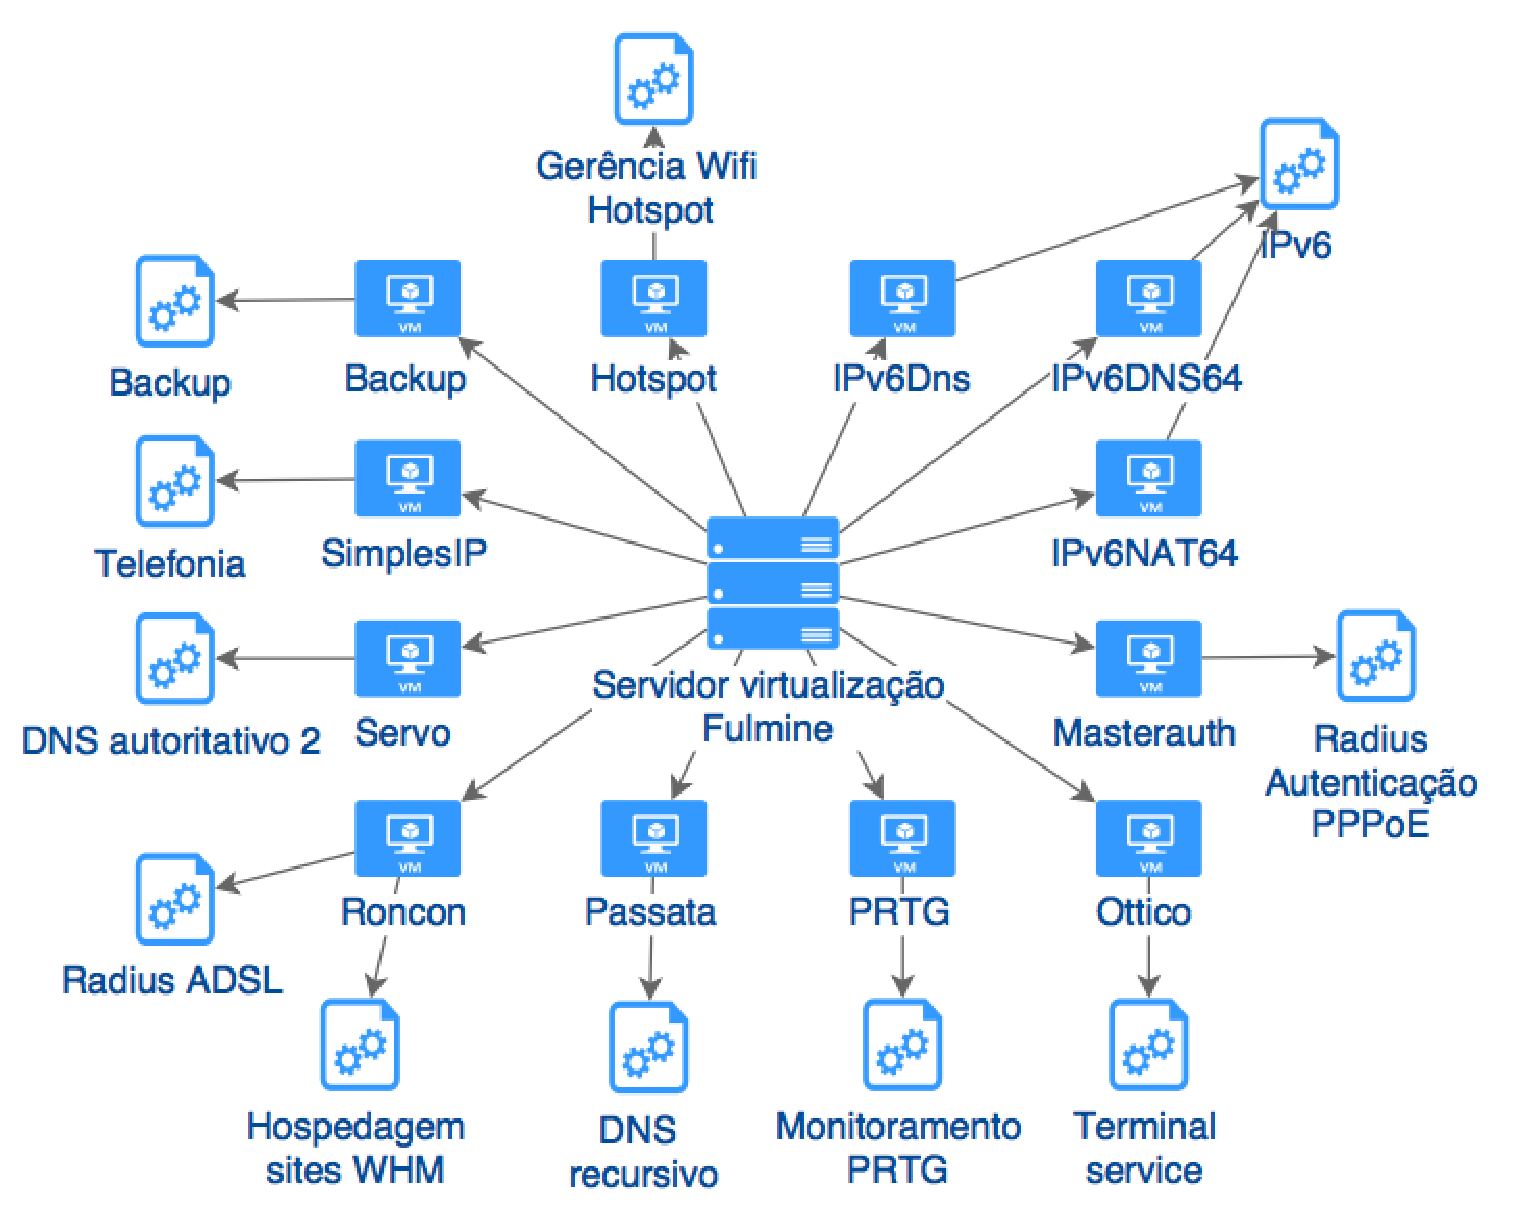
\includegraphics[width=380px]{img/servlog2.eps}
 \caption{Servidor virtualização Fulmine.}
 \label{fig:servlog2}
\end{figure}

Todos os servidores de virtualização possuem o sistema operacional \textit{Ubuntu} versão \textit{14.04 LTS}, para virtualização utiliza-se o 
hipervisor \ac{KVM} e o \textit{QEmu}, ambos são projetos de \textit{software} livre, para compor o ambiente de virtualização...

-graficos cpu memoria disco cada servidor de virtualizacao? colocar aqui ou na implementacao?

A maioria dos serviços são fornecidos por meio de \textit{software} de código aberto, e a maioria dos sistemas operacionais são \textit{Ubuntu}
ou outros sistemas de código aberto, que também são \textit{softwares} livre.

%A Tabela \ref{tab:servporservidor} mostra todos os servidores, incluindo virtuais, e seus respectivos serviços.
%\begin{table}
%\caption {Serviços por servidor}
%\label{tab:servporservidor}
%\begin{center}
%\begin{tabular}{|l|p{12cm}|}\hline
%Servidor & Descrição\\\hline
%asp & Servidor web linguagem ASP\\\hline
%backup & Servidor de backup equipamentos de rede do provedor\\\hline
%bello & Servidor de storage do bacula, para backup dos outros servidores\\\hline
%brina & Servidor de virtualização\\\hline
%cacti & Servidor de monitoramento da rede do provedor\\\hline
%cactibackbone & Servidor de monitoramento da rede do provedor\\\hline
%dati & Banco de dados dos servidores de email e cameras\\\hline
%dio & Servidor de hospedagem de sites PHP4\\\hline
%esibire & Servidor de hospedagem de vídeos\\\hline
%fatefurbo & Servidor para gerência da fibra óptica do provedor\\\hline
%fiberhome & Servidor para gerência da fibra óptica do provedor\\\hline
%fulmine & Servidor de virtualização\\\hline
%hotspot & Servidor de gerência de equipamentos da Ubiquiti que fazem hotspot utilizado pelo provedor\\\hline
%ledriovardar & Servidor de terminal service do suporte e gerência do provedor\\\hline
%masterauth & Servidor de autenticação PPPoE do provedor\\\hline
%merak & Servidor de email\\\hline
%miatanto & Servidor de streaming Icecast para web rádio\\\hline
%mondoperso & Servidor de streaming Icecast de uma rádio ao vivo\\\hline
%monete & Servidor de hospedagem de site dedicada do provedor\\\hline
%monit & Servidor de monitoramento e gráficos de todos servidores\\\hline
%nino & Ambiente de desenvolvimento para setor de programação web\\\hline
%ns & Servidor primário de DNS autoritativo\\\hline
%ottico & Servidor de terminal service do suporte e gerência de fibra óptica do provedor\\\hline
%parla & Servidor de mensagens instantâneas XMPP do provedor\\\hline
%passata & Servidor primário de DNS recursivo do provedor\\\hline
%passata2 & Servidor secundário de DNS recursivo do provedor\\\hline
%piova & Servidor de virtualização\\\hline
%pomodoro & Servidor de documentação Sakai do provedor\\\hline
%postfix & Servidor de SMTP para envio de email marketing\\\hline
%quebei & Servidor de gerência do bacula, para backup dos outros servidores\\\hline
%raggio & Servidor de virtualização\\\hline
%rauco & Servidor de hospedagens WHM\\\hline
%roncon & Servidor de hospedagens WHM\\\hline
%ronconradius & Servidor de radius ADSL de terceiros\\\hline
%servo & Servidor secundário de DNS autoritativo\\\hline
%servo6 & Servidor terciário de DNS autoritativo\\\hline
%sfrunhon & Servidor de gráficos para monitoramento de clientes do provedor\\\hline
%simplesip & Servidor de telefonia Asterisk do provedor\\\hline
%soldi & Servidor de sistemas do provedor e outros ERPs\\\hline
%speedauth & Servidor de autenticação PPPoE do provedor\\\hline
%tempesta & Servidor de virtualização\\\hline
%trapel & Servidor de teste de banda do provedor\\\hline
%tuono & Servidor de virtualização\\\hline
%venti & Servidor de virtualização\\\hline
%vigilante & Servidor de reprodução e armazenamento das câmeras do provedor\\\hline
%vinicolag & Servidor de backup de um cliente\\\hline
%\end{tabular}
%\end{center}
%\end{table}

\section{Serviços críticos}
\label{section:servcrit}



Esboço:\\
-DNS (impacto direto para clientes e rede interna): \\
requisicoes por segundo\\
numero de usuarios\\
-Radius (impacto direto para clientes): \\
numero de usuarios autentidados em x tempo\\
quantidade de dados armazenados no db em x tempo, trafego utilizado, tempo conexao\\
numero de usuarios\\
-Sistemas (impacto indireto para clientes): \\
gasto com funcionarios ociosos\\
quantidade de atendimento a clientes\\
numero de cobrancas enviadas para clientes efetuar pagamento\\
comunicacao entre setores e funcionarios\\
numero de usuarios\\
-Telefonia (impacto indireto para clientes): \\
quantidade de atendimento a clientes\\
comunicacao entre setores e funcionarios\\
ligacoes saintes, atendimento, cobranca, tecnicos instalacoes internet\\
numero de usuarios\\

Exibir disponibilidade média atual dos serviços, com gráficos

